\documentclass[12pt, a4paper, openany]{book}
\usepackage{fstyle}

\graphicspath{ {./img/} }

\begin{document}

\title{Analisi Matematica}
\author{Fabio Ferrario}
\date{2022}
\maketitle

\tableofcontents

\chapter*{Prefazione}
\section{Introduzione}
Questi appunti di Analisi Matematica sono stati fatti con l'obiettivo di riassumere tutti (o quasi) gli argomenti utili per l'esame di Analisi Matematica del corso di Informatica dell'Università degli Studi di Milano Bicocca.
\\Come fonte ho utilizzato:
\begin{itemize}
	\item Appunti di altri studenti
	\item Libro "Analisi Uno, teoria ed esercizi" di Giuseppe De Marco (terza edizione)
\end{itemize}
\section*{Il Corso}
Come già detto, questi appunti sono in funzione del corso di Analisi Matematica di UNIMIB, a.a. 2021/22, insegnato dalla Professoressa Pini.
\subsection*{Programma del corso}
\begin{enumerate}
	\item Numeri Reali
	      \begin{enumerate}
		      \item Funzioni elementari
		      \item Generalità sulle funzioni
		      \item Funzioni reali di una variabile
	      \end{enumerate}
	\item Successioni
	      \begin{enumerate}
		      \item Limiti di successioni reali
		      \item Principio di Induzione
		      \item Limiti notevoli
	      \end{enumerate}
	\item Limiti e continuità
	      \begin{enumerate}
		      \item Limiti di Funzioni
		      \item Limiti notevoli
		      \item Funzioni continue
		      \item Proprietà globali delle funzioni continue
	      \end{enumerate}
	\item Calcoli differenziale
	      \begin{enumerate}
		      \item Derivate di una funzione
		      \item Proprietà delle funzioni derivabili
		      \item Funzioni convesse e concave
		      \item Formula di Taylor
		      \item Grafici di funzioni
	      \end{enumerate}
	\item Calcolo integrale
	      \begin{enumerate}
		      \item Funzioni integrabili secondo Rienmann
		      \item Teorema fondamentale del calcolo e integrali indefiniti
		      \item Metodi d'integrazione
	      \end{enumerate}
	\item Serie numeriche
	      \begin{enumerate}
		      \item Serie, convergenza, convergenza assoluta
		      \item Serie a termini positivi
		      \item Serie a termini di segno variabile
	      \end{enumerate}
\end{enumerate}

\subsection*{Prerequisiti}
\emph{Algebra elementare}: Calcolo letterale, equazioni e disequazioni di primo e secondo grado
\\\emph{Trigonometria elementare}
\\\emph{Esponenziali e logaritmi}

\chapter{Analisi 0}
\paragraph{introduzione}
Questa piccola sezione contiene alcuni argomenti che non fanno parte del programma di Analisi matematica ma possono essere propedeutici ad essa.
\section{Linguaggio della matematica }
La matematica è fatta di:
\begin{itemize}
	\item Definizioni $\leftarrow$ Circoscrive un campo, in modo da definire se un oggetto vi appartiene o no
	\item Assiomi/Postulati $\leftarrow$  Affermazione che viene accettata come vera senza che essa venga dimostrata
	\item Preposizioni/Teoremi $\leftarrow$  un teorema è struttrato così: data questa premessa (ipotesi) è possibile dedurre delle conseguenze (tesi)
\end{itemize}
\paragraph*{Affermazioni} In matematica se affermo "Se \emph{un} numero è divisibile per 6, allora lo è anche per due", quel "un" in matematica si traduce in \emph{"esiste un numero"} oppure in \emph{"per ogni numero"}
\begin{itemize}
	\item $\forall \leftarrow$ Per ogni
	\item $\exists \leftarrow$ Esiste
\end{itemize}

\paragraph*{Proposizioni}
Le proposizioni in matematica sono fatte da soggetto + predicato nominale e possono risultare Vere o False.
esempio:
\\Ogni giorno piove (x = giorno e P(x) = piove) $\leftarrow \forall x P(x)$
\\Non ($\forall x P(x)$) $\leftarrow \exists x : \not P(x)$

\paragraph*{Implicazioni}
A e B due proposizioni. Cosa significa A -> B? (a implica b)
\begin{itemize}
	\item A è sufficiente per B
	\item B è necessario per A
\end{itemize}
Ogni triangolo èquilatero è isoscele
\begin{itemize}
	\item Affinchè un triangolo abbia 2 lati uguali è sufficiente che ne abbia tre uguali
	\item Affinchè un triangolo abbia 3 lati uguali è necessario che ne abbia due uguali tra loro
\end{itemize}
Quindi A è ipotesi, B è la tesi.
\section{Disequazioni}
Nel corso di Analisi Matematica troviamo spesso delle disequazioni da risolvere, è bene quindi sapere come risolverle.
In caso non si sia presa in mano la matematica per un po di tempo, potrebbe essere una buona idea ripassarle.

\paragraph*{Le disequazioni} sono come delle equazioni in cui ci si chiede "per quali valori di $x$ questa espressione è maggiore (minore) di un certo valore".
Vengono risolte esattamente come le equazioni, ma il significato del risultato è diverso.

\subsection{Disequazioni di secondo grado}
Le disequazioni (come le equazioni) di secondo grado si risolvono, una volta ridotte alla forma standard $ax^2+bx+c$, usando la formula risolutiva:
$$x_{1 2} = \frac{-b\pm\sqrt{b^2-4ac}}{2a}$$
A seconda del valore di $\Delta = b^2-4ac$, la disequazione (equazione) ammette:
\begin{itemize}
	\item $\Delta > 0 \implies $ 2 soluzioni Reali
	\item $\Delta < 0 \implies $ Nessuna soluzione Reale (ma 2 complesse)
	\item $\Delta = 0 \implies $ 1 Soluzione Reale
\end{itemize}
Ricordiamo poi, che una funzione del tipo $y=ax^2 +bx +c$ è una \emph{parabola}, quindi con una disequazione (ponendo $f(x)>0$) ci si chiede semplicemente per quali valori di $x$ la funzione è maggiore di 0,
quindi quando sta sopra l'asse delle ascisse.
\paragraph*{}
Il $\Delta$, e il valore del parametro $a$ della funzione determinano la "rappresentazione" della parabola
\\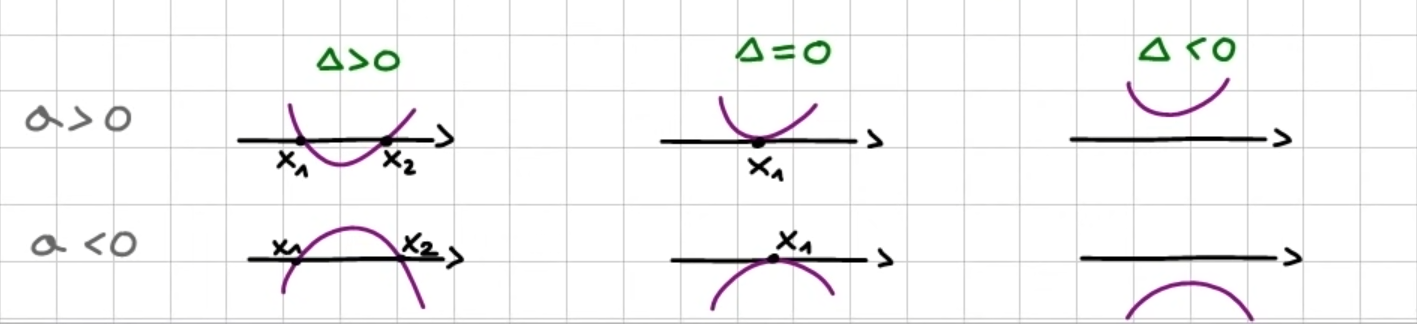
\includegraphics[width=\textwidth]{parabole-delta.png}

\paragraph*{Legge di annullamento del prodotto}
Segnare sta cosa

\subsection*{Disequazioni con valore assoluto}
Quando troviamo una disequazione con valore assoluto, bisogna porre a sistema la disequazione con \emph{l'argomento del modulo posto prima maggiore, poi minore di zero}.
Così facendo avremo due sistemi di disequazioni, che risolti separatamente ci daranno i due risultati della disequazione
\esempio{
	$|2x-3| > x + 6$. Dobbiamo eliminare il valore assoluto.
	\\quindi ponendo l'argomento del modulo \emph{maggiore o uguale a zero}:
	\begin{equation*}
		\begin{cases}
			2x-3 \geq 0 \\
			2x-3 > x+6
		\end{cases}
		=
		\begin{cases}
			x\geq \frac{3}{2}\\
			x > 9
		\end{cases}
		= x>9
	\end{equation*}
	E ponendolo \emph{minore di zero} (nota che cambia di segno):
	\begin{equation*}
		\begin{cases}
			2x-3 < 0 \\
			-2x+3 > x+6
		\end{cases}
		=
		\begin{cases}
			x < \frac{3}{2}\\
			x < -1
		\end{cases}
		= x<-1
	\end{equation*}
	Quindi il risultato è: $x>9 \vee x<-1$
}
\section{Richiamo di trigonometria}
un piccolissimo richiamino di trigonometria (DA COMPLETARE)
\begin{itemize}
	\item $\frac{\cos(x)}{\sin(x)} = \cot(x)$
\end{itemize}
\paragraph*{Valori di $\sin(x)$}
\begin{itemize}
	\item $\sin(0) = 0$
	\item $\sin(\pi/2) = 1$
	\item $\sin(\pi) = 0$
\end{itemize}
\paragraph*{Valori di $\cos(x)$}
\begin{itemize}
	\item $\cos(0) = 1$
	\item $\cos(\pi/2) = 0$
	\item $\cos(\pi) = -1$
\end{itemize}
\section{Valore assoluto (modulo) di un numero Reale}

\definizione{ Per ogni $x \in R$ si pone
	\begin{equation}
		|x| = \begin{cases}
			x  & \text{se $x \geq 0$} \\
			-x & \text{se $x < 0$}
		\end{cases}
	\end{equation}
	$|x|$ si dice valore assoluto, o modulo, di x
}
\paragraph{ATTENZIONE} dire che "il modulo di un numero è il numero senza il segno" non ha senso in questo contesto, quindi non va usata perchè vale solo se x è "semplice"
\paragraph{In parole povere} il modulo di $x$ è $x$ se x è positivo, il suo opposto se è negativo\\
quindi $|3 - \pi| = \pi - 3$ perchè $3-\pi$ è negativo ($3 - 3.14$) quindi il suo modulo è il suo opposto.
\\Volendo, $|x|$ si può anche interpretare come il massimo tra $x$ e $-x$.

\paragraph{Modulo e moltiplicazione}
Per ogni $x, y \in R$ si ha $|xy| = |x||y|$.\\Se $y\neq0$, si ha anche $|x/y|=|x|/|y|$
\paragraph{Modulo e addizione}
Il modulo della somma NON coincide con la somma dei moduli. Però vale la seguente importantissima disuguaglianza:
\paragraph{Disuguaglianza triangolare} siano x,y numeri reali. Allora:
\begin{equation}
	|x+y| \leq |x| + |y|
\end{equation}
(cioè il modulo della somma è minore o uguale della somma dei due moduli)

\section{Insiemi e Intervalli in R}
\definizione{
	Diremo \textbf{intervallo} di $\R$ un sottoinsieme $I$ di $\R$ che sia convesso rispetto all'ordine, cioè che soddisfi la seguente condizione:
	se $a,b \in I$, e $a \leq b$, ogni $x\in R$ tale che $a \leq x \leq b$ appartiene a $I$.
}

In parole povere: $I$ è intervallo di $\R$ se, contenendo due numeri reali, contiene anche \emph{tutti i numeri reali che stanno fra questi due}.

\paragraph{Intervalli limitati.}
Fissati $a, b \in R$, con $a<b$, si riconosce facilmente che sono intervalli i seguenti sottoinsiemi di $\R$:
\begin{itemize}
	\item[] $[a,b] = \{x \in R : a \leq x \leq b\}$ CHIUSO
	\item[] $[a,b) = \{x \in R : a \leq x < b\}$ SUPERIORMENTE APERTO
	\item[] $(a,b] = \{x \in R : a > x \leq b\}$ INFERIORMENTE APERTO
	\item[] $(a,b) = \{x \in R : a > x < b\}$ APERTO
\end{itemize}
{\tiny(le parentesi tonde a volte vengono sostituite con delle parentesi quadre nel senso opposto)}
\\Tutti questi intervalli sono detti intervalli \emph{limitati}
\paragraph{Intervalli illimitati.} sono invece intervalli illimitati, per ogni $a \in R$, gli insiemi:
\begin{itemize}
	\item[] $\{x \in R: x \geq a\}$ (semiretta \emph{chiusa} inferiormente limitata)
	\item[] $\{x \in R: x > a\}$ (semiretta \emph{aperta} inferiormente limitata)
	\item[] $\{x \in R: x \leq a\}$ (semiretta \emph{chiusa} superiormente limitata)
	\item[] $\{x \in R: x < a\}$ (semiretta \emph{aperta} superiormente limitata)
\end{itemize}

\subsection*{Massimi e Minimi dei sottoinsiemi di $\R$}
\paragraph{Definizione.} Sia $S$ un sottoinsieme di $\R$. Un elemento $m\in R$ si dice \emph{massimo} di S se appartiene ad S ed è maggiore o uguale di ogni elemento di $S$.
\\Dualmente, $\mu \in \R $ è detto \emph{minimo} di $S$ se appartiene ad $S$ ed è minore o uguale di ogni elemento di $S$
\\Un sottoinsieme può \emph{avere o non avere massimo}, \emph{avere o non avere minimo}, ma se esistono sono UNICI

\subsection*{Maggioranti, minoranti. Insiemi superiormente/inferiormente limitati e limitati}
\paragraph{Definizioni.} Sia $S$ sottoinsieme non vuoto di $\R$. si dice che $b\in \R$ è un \emph{maggiorante} per $S$ se risulta $s\leq b$ per ogni $s \in S$. Si dice che $S$ è \emph{Superiormente limitato} (in $\R$) se ammette maggioranti in $\R$.
\\l'insieme dei maggioranti in $\R$ di $S\subseteq \R$ è indicato con $S^*$.
\\dualmente per i minoranti, ovviamente i minoranti sono tutti minori di $S$ e l'insieme dei minoranti si indica con $S_*$.
\\Un insieme non vuoto $S \subseteq \R$ si dice \emph{limitato} se è tanto superiormente limitato quanto inferiormente limitato.
\subsection*{Prodotto Cartesiano}
\paragraph{Definizione.}Dati due insiemi $X$ e $Y$, il loro prodotto cartesiano è per definizione l'insieme $X \times Y$ formato da tutte le coppie ordinate $(x,y)$ che hanno la prima componente $x \in X$, la seconda $y \in Y$.\\
Se $X = Y$, il prodotto $X \times X$ si chiama \emph{quadrato cartesiano} di $X$ e si indica anche con $X^2$

\chapter{Funzioni}

\section{Generalità}
\definizione{
	Siano $X$ e $Y$ insiemi. Si dice che è data una funzione di $X$ in $Y$, se è data una regola che a ogni elemento di $X$ associa \emph{uno e uno solo} elemento di $Y$.
}
\paragraph{In altre parole} assegnare una funzione $f$ di $X$ in $Y$ significa dare un procedimento che consenta di assegnare a ogni $x \in X$ un ben determinato $y \in Y$. Tale $y$, corrispondente di $x$ tramite la funzione $f$, si indica con $f(x)$, cioè $y = f(x)$ e $y$ si chiama \emph{immagine di $x$ secondo $f$}. per indicare che $f$ è funzione di $X$ in $y$ si scrive $f: X \rightarrow Y$.

\definizione{
	se $f: X \rightarrow Y$ è una funzione, gli insiemi \emph{$X$ e $Y$} sono rispettivamente il \textbf{dominio} e il \textbf{codominio} di $f$.
}
\paragraph{Assegnare una funzione} significa assegnare:
\begin{itemize}
	\item Un dominio $X$
	\item Un codominio $Y$
	\item Una regola che a ogni $x$ del dominio associ una $y$ del codominio
\end{itemize}
Pertanto: due funzioni $f$ e $g$ sono \textbf{uguali} se e solo se hanno lo \emph{stesso dominio}, lo\emph{ stesso codominio}, e inoltre si ha \emph{$f(x) = g(x)$ per ogni x del dominio}.\\
Non basta dunque dire che la regola sia la stessa: occorre anche che il dominio e il codominio dati siano gli stessi.

\subsection*{Insieme immagine}
Se $f: X \rightarrow Y$ è una funzione, ed $S$ è sottoinsieme del dominio $X$ (cioè $S \subseteq X$) si indica con $f(s)$ l'insieme degli elementi $y$ che sono immagini secondo $f$ di qualche elemento di $S$.
In linguaggio matematico è $f(S) = \{ f(x) : x \in S\}$ oppure si può anche descrivere così: $f(S) = \{y \in Y : \exists x \in S \text{ tc } y = f(x)\}$.
L'insieme $f(S)$ è detto \emph{immagine di $S$ tramite $f$}; per $S = X$ (quindi se S corrisponde col dominio), $f(X)$ è detto \emph{immagine di f}.
Vale sempre $f(X) \subseteq Y$, quindi l'immagine è \emph{sempre} conenuta nel codomino, ma in generale è $f(X) \subset Y$, cioè immagine e codominio sono diversi.
\paragraph{In parole povere} L'insieme immagine di una funzione è l'insieme di tutti i valori della funzione per ogni elemento del dominio.
L'insieme immagine è \emph{sempre} contenuta nel dominio, ma non sempre vi coincide.

\subsubsection{Immagine Inversa}
Dualmente al concetto di immagine c'è quello di antiimmagine.
\paragraph{Definizione. }Sia $\function $ una funzione, sia $F \subseteq Y$.
Si chiama immagine inversa $f^\leftarrow(T)$ (o controimmagine, o antiimmagine) di $T$ mediante $f$ l'insieme degli $x \in X$ la cui imamgine sta in $T$.
in simboli: $f^\leftarrow(T) = \{ x \in X : f(x) \in T\}$.
\paragraph{In parole povere} L'antiimmagine mediante un insieme $T$ è l'insime dei valori del dominio la cui immagine è contenuta in $T$


\section{Composizione di Funzioni}
Siano $\function$ e $g: Y \rightarrow Z$ funzioni.
Si ottiene una funzione $g \circ f : X \rightarrow Z $ (che si legge "g tondo f" o "g cerchietto f") ponendo $g \circ f = g(f(x))$ per ogni $x \in X$;
$g \circ f$ è detta \emph{funzione composta} di f e g; è la funzione ottenuta applicando $f$ e $g$ nell'ordine.
\\Per poter fare la composizione, \textbf{occorre che il codominio di $f$ coincide con il dominio di $g$}.


\esempio{
	Siano $f: \mathbf{R} \rightarrow \mathbf{R}$ e $g: \mathbf{R} \rightarrow \mathbf{R}$ due funzioni così definite:
	\\ $f(x) = x^2$ e $g(x) = x - 2$ allora $f \circ g = f(g(x)) = (x-2)^2$
}
\section{Iniettività e Suriettività}

\subsection*{Funzioni Suriettive}
Quando l'\emph{insieme immagine e il codomino di una funzione coincidono}, essa si dice che è \emph{suriettiva}
\definizione{Una funzione $\function$ si dice \textbf{suriettiva} se è $f(X) = Y$.
	Attenzione che su alcuni testi di Analisi il termine codominio è inteso nel senso di immagine.}

\subsection*{Funzioni Iniettive}
La funzione $\function$ è detta \textbf{iniettiva} se trasforma elementi distinti in elementi distinti, ovvero:
\definizione{$f: X \rightarrow Y$ si dice iniettiva se per ogni $x_1, x_2 \in X$ e $x_1 \neq x_2$ implicano $f(x_1) \neq f(x_2)$.}
\paragraph{}Per vedere che una $\function$ \emph{non} è iniettiva, basta esibire anche una sola coppia $x_1, x_2$ di elementi distinti ($x_1 \neq x_2$) del dominio per cui sia $f(x_1) = f(x_2)$.
\\Per provare invece che è iniettiva, occorre dimostrare che per ogni coppia di elementi distinti $x_1, x_2 \in X, x_1 \neq x_2$ si ha $f(x_1) \neq f(x_2)$

\subsubsection{Biiezioni}
Una funzione $\function$ è detta biiettiva se è sia iniettiva che suriettiva.
Quindi $\function$ è biiettive se e solo se per ogni $y \in Y$ esiste uno e un solo $x \in X$ tale che sia $y = f(x)$.
Che esista almeno un tale $x$ dice che $f$ è suriettiva, che sia unico dice che $f$ è iniettiva.
Una funzione biiettiva viene detta anche biiezione e corrispondenza biunivoca.

\subsection*{Funzione Inversa}
Se $\function$ è biiettiva, si può definire una funzione inversa di $f$,$f^{-1} : Y \rightarrow X$, nel modo seguente:
dato $y \in Y$, $f^{-1}(y)$ è quell'unico $x \in X$ tale che sia $y = f(x)$.
se $\function$ non è biiettiva, la funzione inversa di f non può essere definita.
\paragraph*{} se $f$ è funzione reale di variabile reale biiettiva, il grafico dell'inversa $f^{-1}$ si ottiene facendo il simmetrico del grafico di $f$ rispetto alla retta di equazione $x=y$.

\section*{Funzioni Pari/Dispari}
Sia $\function$ una funzione reale di variabile reale (quindi $X, Y in \R$).
\paragraph*{Pari}
Si dice che $f$ è pari se per ogni $x \in X$ anche $-x \in X$ ed è $f(x) = f(-x)$;
\\Le funzioni pari hanno grafico simmetrico rispetto all'asse delle ordinate.
\paragraph*{Dispari}
Si dice che $f$ è dispari se per ogni $x \in X$ anche $-x \in X$ ed è $f(x) = -f(x)$;
\\Le funzioni dispari hanno grafico simmetrico rispetto all'origine

\section{Monotonia di una Funzione}
Sia $\function$ una funzione reale di variabile reale (quindi $X, Y in \R$).

\subsection*{Funzione Crescente}
Si dice che $f$ è \emph{crescente} se da $x_1, x_2 \in X$ e $x_1 < x_2$ segue $f(x_1) \leq f(x_2)$;
\\Se invece $x_1, x_2 \in X$ e $x_1 < x_2$ implicano $f(x_1) < f(x_2)$ allora $f$ si dice \emph{strettamente crescente};

\subsection*{Funzione Decrescente}
Si dice che $f$ è \emph{decrescente} se da $x_1, x_2 \in X$ e $x_1 > x_2$ segue $f(x_1) \geq f(x_2)$;
\\Se invece $x_1, x_2 \in X$ e $x_1 < x_2$ implicano $f(x_1) > f(x_2)$ allora $f$ si dice \emph{strettamente decrescente};

\paragraph{Come si calcola la monotonia?}
Per calcolare la monotonia di una funzione, bisogna porre la derivata (che è il "rateo" di crescita della funzione) \emph{Maggiore (o minore o maggiore uguale o minore uguale) di 0}.
Nei punti in cui la derivata rimane maggiore (minore,...) di 0, la funzione è \emph{monotona crescente (decrescente,...)}


\section{Studio di Funzione}
Una parte importantissima dell'Analisi Matematica (che fa parte di un intero esercizio d'esame) è lo \emph{Studio di Funzione},
che mette insieme quasi tutti gli argomenti del corso.

Lo studio di funzione è composto di 5 passaggi:
\begin{enumerate}
	\item Definizone del Dominio
 \item Segno e intersezione con gli assi
 \item Limiti e Asintoti
 \item Segno della derivata
\end{enumerate}

\subsection{Definizione del Dominio}
Una funzione $f:\R \to \R$ non sempre è definita in tutto $\R$, spesso ci sono degli intervalli (o dei punti) in cui non è definibile.
Per trovare questi punti in cui non è definibile bisogna:
\begin{itemize}
	\item porre tutti i \textbf{Denominatori $\neq 0$}
 \item porre tutti gli \textbf{Argomenti delle Radici pari $\geq 0$}
 \item porre tutti gli \textbf{Argomenti dei Logaritmi $>0$}
 \item ogni funzione del tipo $f(x)^{g(x)}$, $f(x)$ va posto maggiore di 0
 \item gli argomenti di $\arcsin$ e $\arccos$ vanno posti $-1 < x <1$
\end{itemize}
Ovviamente, una volta definito il dominio della funzione vado a eliminare dal piano cartesiano le zone in cui $f(x)$ non è definita.
\subsection*{Simmetrie/Periodicità}
Questa fase è facoltativa ma ogni tanto ci aiuta.
\begin{equation}
	f(-x) = \begin{cases}
		f(x) \implies \text{Funzione Pari}\\
		-f(x) \implies \text{Funzione Dispari}\\
		NIL \implies \text{Funzione ne Pari ne Dispari}
	\end{cases}
\end{equation}
Le \emph{Funzioni Periodiche} sono generalmente quelle goniometriche.
\subsection{Segno e Intersezione con gli Assi}
Il segno della funzione ci permette di vedere dove la funzione è positiva.
L'intersezione con gli assi invece ci aiuta a disegnare la funzione.
\begin{itemize}
	\item $f(x)\geq 0$ Per vedere dove la funzione è positiva
 \item $f(x)=0$ è l'intesezione con l'asse delle ascisse
 \item $f(0)$ è l'intersezione con l'asse delle ordinate
\end{itemize}

\subsection{Limiti e asintoti}
I limiti ci servono a capire come si comporta la funzione ai limiti del dominio e nei punti di disconitinuità.
Bisogna calcolare i limiti di x ai punti di accumulazione del dominio che non fanno parte del dominio e agli estremi di esso.

\begin{itemize}
	\item Se $x_0 \notin DOM$ e $\limite{x}{x_0} f(x) = c \implies$ il grafico ha un "buco" in $(x_0,c)$.
 \item Se $x_0 \notin DOM$ e $\limite{x}{x_{0}^\pm} f(x) = \pm \infty \implies$ $x=x_0$ è asintoto VERTICALE.
 \item Se $\limite{x}{\pm \infty} = l$ l è asintoto ORIZZONTALE
 \item Se $\limite{x}{\pm \infty} = \pm \infty$ potrebbe eistere Asintoto Obliquo
\end{itemize}
\subsection{Segno della Derivata}
Tramite il segno della derivata, si determina la Crescenza/Decrescenza della funzione.
Ponendo la derivata $>0$ si trovano gli intervalli in cui la funzione è crescente.

\chapter{Successioni}

\section{Introduzione}
\definizione{
	Una \emph{Successione di numeri reali} è una funzione $a: \N \to \R$.\\
	La variablie Indipendente viene di solito indicata con $n$ mentre per la funzione alla notazione $a(n)$ si preferisce $a_n$
}
\esempio{
	$a_n = 2n-3$ è una successione.
	$a_0 = -3$, $a_1 = -1$, $a_2 = 1$, $a_3 = 3$ , ... sono i suoi valori
}

\paragraph*{Limitazioni} Una successione $\{a_n\}$ si dice:
\begin{itemize}
	\item \textbf{Inferiormente limitata} se esiste $m \in \R$ tale che $a_n \geq m \forall n \in \N$
	\item \textbf{Superiormente limitata} se esiste $M \in \R$ tale che $a_n \leq M \forall n \in \N$
	\item \textbf{Limitata} se esistono $m \in \R$ e $M \in \R$ tali che $m \leq a_n \leq M \forall n \in \N$
\end{itemize}
\esempio{
	La successione $\{\frac{1}{n+1}\}$ i cui primi termini sono $1, \frac{1}{2}, \frac{1}{3},$...\\
	è \emph{limitata}: si ha infatti che $0 < a_n \leq 1 \forall n \in \N$
}

\paragraph*{Monotonia} Una successione $\{a_n\}$ si dice:
\begin{itemize}
	\item \textbf{Monotona crescente} se $a_n\leq a_{n+1} \forall n \in \N$
	\item \textbf{Monotona strettamente crescente} se $a_n < a_{n+1} \forall n \in \N$
	\item \textbf{Monotona decrescente} se $a_n \geq a_{n+1} \forall n\in\N$
	\item \textbf{Monotona strettamente decrescente} se $a_n > a_{n+1} \forall n \in \N$
\end{itemize}

\paragraph*{Definizione} Si dice che una successione {$a_n$} possiede (o acquista) una certa proprietà \textbf{definitivamente} se esiste $N \in \N$ tale che
$a_n$ soddisfa quella proprietà per ogni $n \geq N$, quindi da un certo $n$ in poi.

\esempio{Queste serie:\\
	$a_n = 2n-3$ $[-3,-1,1,3,5,...]$  è \emph{Definitivamente positiva}\\
	$a_n =\frac{1}{n+1}$ $[1, \frac{1}{2}, \frac{1}{3},\frac{1}{4}...] $ è \emph{Definitivamente minore di $\frac{1}{3}$}
}

\section{Limiti di Successioni}
\paragraph*{}Calcolare il limite di una successione (che si indica con $\limite{n}{+\infty}a_n$ o $\lim a_n$)
è equivalente a chiedersi che tipo di comportamento ha la successione quando $n$ tende a diventare molto molto grande.

\paragraph*{Definizione} Sia $a_n$ una successione, e sia $l \in \R$.
Si dice che $a_n$ ha per limite $l$ per $n$ tendente all'infinito (o che $a_n$ tende a $l$)
se la successione $a_n$ si trova \emph{definitivamente} in ogni intorno di $l \in \R$
e si scrive $\limite{n}{+\infty} a_n = l$

Quando si calcola il limite bisogna però distinguere 4 casistiche:
\begin{enumerate}
	\item \textbf{Convergenza}, se $l\in\R$, si ha $\lim a_n = l$ sse $\forall \epsilon > 0$ esiste un indice $n_\epsilon\in\N$ tale che si abbia:
	      \begin{center}
		      $|a_n-l|\leq\epsilon$ per ogni $n \geq n_\epsilon$
	      \end{center}
	\item \textbf{Divergenza a $+\infty$}, si ha $\lim a_n = +\infty$ sse $\forall a\in \R$ esiste un indice $n_a\in\N$ tale che si abbia:
	      \begin{center}
		      $a_n\geq a$ per ogni $n \geq n_a$
	      \end{center}
	\item \textbf{Divergenza a $-\infty$}, si ha $\lim a_n = -\infty$ sse $\forall a\in \R$ esiste un indice $n_a\in\N$ tale che si abbia:
	      \begin{center}
		      $a_n\leq a$ per ogni $n \geq n_a$
	      \end{center}
	\item \textbf{Indeterminazione} se non si verifica nessuno dei casi precedenti, quindi il $\lim a_n$ non esiste.
\end{enumerate}
\paragraph*{In parole povere} La successione converge se la successione al crescere di n va ad avvicinarsi sempre di più a $l$,
diverge a $+\infty$ se esiste un indice che permette alla successione di essere più grande di un qualsiasi numero Reale
e infine diverge a $-\infty$ se esiste un indice che permette alla successione di essere più piccolo di una qualsiasi numero Reale.
\subsection*{Teorema di esistenza del limite}
\definizione{
	Se una successione è monotona crescente allora il limite esiste e coincide con l'estremo superiore della successione.
	Se invece è monotona decrescente allora il limite esiste e coincide con l'estremo inferiore della successione.
}
\section{Principio di Induzione}
\subsection*{Introduzione}
Il principio di Induzione è un teorema noto, che è spesso utile per discutere la validità di una successione \emph{infinita} di proposizioni in un \emph{numero finito di passi}.

\definizione{
	Sia data una proposizione $P(n)$, $\forall n \in \N$ con $n > n_0$ .
	\\Se sono soddisfatte le seguenti condizioni:
	\begin{enumerate}
		\item $\exists n_0$ tale che $P(n_0)$ è VERA
		\item $\forall n \geq n_0$ vale l'implicazione $P(n-1) \implies P(n)$
	\end{enumerate}
	\emph{Allora $P(n)$ è vera per ogni $n \geq n_0$}
}
\paragraph*{}
Una \emph{propisizione} è un qualunque enunciato il cui valore dipende da $n$, per esempio "$n$ è pari", "$n$ è primo".

\esempio{
	Consideriamo l'enunciato: $P(n): 2^n \geq n^3$,
	e proviamo che "$P(n)$ vera $\implies P(n+1)$ vera" per ogni $n\geq 7$.
	Infatti per $n \geq 7$ risulta:
	\begin{equation*} %TODO vai a capire cosa vuol dire sta roba
		2^{n+1} = 2\cdot 2^n \geq 2 \cdot n^3 = n^3 + n \cdot n^2 \geq n^3 + 7n^2 \geq n^3 + 3n^2 +3n+1 = (n+1)^3
	\end{equation*}
	e quindi per ogni $n \geq 7$, se $2^n \geq n^3$ allora $2^{n+1} \geq (n+1)^3$.
	D'altra parte, semplici calcoli mostrano che $P(n)$ è falsa per $n = 7,8,9$, mentre è vera per $n=10$.
	Sintetizzando si può dire che $P(n)$ è \emph{induttiva}, cioè verifica l'implicazione, per ogni $n \geq 7$, mentre è vera per ogni $n \geq 10$, dal momento che (1) è verificata con $n_0=10$.
}

\esempio{ \emph{Somma di Gauss}\\
	Proviamo per induzione che $\forall n\in\N$ risulta:
	\begin{equation*}
		P_n: \sum_{k=0}^n k= \frac{n(n+1)}{2}
	\end{equation*}
	ovvero, la somma dei primi $n \in\N$ numeri equivale a $\frac{n(n+1)}{2}$
	\paragraph*{}Questa formula è banalmente vera per $n=0$.
	Mentre per il passo induttivo si può provare come segue:
	\begin{equation*}
		\sum_{k=0}^{n+1} k = \sum_{k=0}^{n} k + (n+1) = \frac{n(n+1)}{2} + (n+1) = \frac{(n+1)(n+2)}{2}
	\end{equation*}
	\paragraph*{Spiegazione}
	se guardi $\frac{(n+1)(n+2)}{2}$ si può notare che equivale a $\frac{n(n+1)}{2}$ se ad $n$ sostituisci $n+1$
	%TODO trovare un modo migliore per spiegare sta roba mannaggia a te
}

\esempio{
Un esempio sostanzialmente analogo è il seguente:\\
\begin{equation*}
	P_n: \sum_{k=0}^n x^k = \frac{1-x^{n+1}}{1-x}
\end{equation*}
\paragraph*{}Questa formula è banalmente vera per $n=0$.
Mentre per il passo induttivo si può provare come segue:
\begin{equation*}
	\sum_{k=0}^{n+1} x^k = \sum_{k=0}^n x^k \cdot x^{n+1} = \frac{1-x^{n+1}}{1-x}\cdot x^{n+1} = \frac{1-x^{n+2}}{1-x}
\end{equation*}
\paragraph*{Spiegazione} Osserviamo che $\frac{1-x^{n+2}}{1-x}$ equivale a $\frac{1-x^{n+1}}{1-x}$ sostituendo $n$ con $n+1$
}

\chapter{Limiti e Continuità}

\section{Forme di Indecisione}
Le forme di Indecisione (o forme indeterminate) sono operazioni che coinvolgono infiniti e infinitesimi nel calcolo dei limiti per le quali \emph{non è possibile determinare un risultato a priori}.
\\Le operazioni problematiche nel calcolo dei limiti sono essenzialmente sette:
\begin{center}
	$[\frac{0}{0}]$ $[\frac{\infty}{\infty}]$ $[1^\infty]$ $[\infty - \infty]$ $[0^0]$ $[\infty^0]$
\end{center}

\section{Limiti Notevoli}
\begin{itemize}
	\item $\limite{x}{0} \ln(1+x) \sim x$
	\item $\limite{x}{0} \ln(1-x) \sim -x$
\end{itemize}



\section{Asintoti Verticali e Orizzontali}
\subsection*{Asintoti Verticali}
\definizione{
	Si dice che la retta $x=a$ è un \emph{Asintoto Verticale} di $f(x)$ se si verifica almeno una di queste caratteristiche:
	\begin{itemize}
		\item $\limite{x}{a^-} f(x)= +\infty$
		\item $\limite{x}{a^-} f(x)= -\infty$
		\item $\limite{x}{a^+} f(x)= +\infty$
		\item $\limite{x}{a^+} f(x)= -\infty$
	\end{itemize}
	Una funzione può avere un numero qualsiasi di asintoti verticali
}
\paragraph*{In poche parole} Un Asintoto Verticale è una retta che fa da "muro" nel dominio di una funzione, e si trova facendo il limite della funzione in un punto specifico, se questo limite è uguale a $\pm \infty$ allora abbiamo trovato un asintoto verticale.

\paragraph*{Come si trova??} Per trovare eventuali \emph{Asintoti Verticali} devo identificare i punti dove ci sono \emph{problemi di definizione},
come "buchi" o estremi del dominio.

\esempio{
	$$y = \ln x + \frac{1}{x-2}$$
	Dominio: $x-2 \neq 0 \rightarrow x\neq 2 \wedge x>0$
	\\In questo esempio abbiamo dei problemi di definizione in $x=2$, dove c'è un "buco" nel dominio, e in $x=0$ dove c'è il limite del dominio.
	\\in questi punti \emph{potrebbero} esserci degli AV. Proviamo:
	\\$\limite{x}{0^+} f(x)= -\infty$
		\\$\limite{x}{2^-} f(x)= -\infty$
	\\$\limite{x}{2^+} f(x)= +\infty$
		\\Quindi $x=0$ e $x=2$ sono asintoti verticali.
}
\subsection*{Asintoti Orizzontali}
Una situazione abbastanza analoga la si ha con gli \emph{Asintoti Orizzontali}
\definizione{
	Si dice che la retta $y=l$ è un \emph{Asintoto orizzontale (destro)} di $f(x)$ per $x\to +\infty$ se $\limite{x}{+\infty} f(x) = l$
	\\Si dice che la retta $y=l$ è un \emph{Asintoto orizzontale (sinistro)} di $f(x)$ per $x\to -\infty$ se $\limite{x}{-\infty} f(x) = l$

}
In questo caso però, una funzione può avere \emph{al massimo 2 asinto   ti orizzontali}

\section{Asintoti Obliqui}
\paragraph*{definizione}{ %la definizione è broken, va sistemata TODO
	Si dice che la retta $y=mx + q$ è un asintoto obliquo (destro) di $f(x)$ per $x \to +\infty$ se
	$\limite{x}{+\infty} [f(x)-mx-q]=0$.
	Una Situazione analoga lo si ha per $-\infty $ (sinistro).
}

Una funzione può avere al massimo 2 asintoti obliqui diversi, uno a $+\infty$ e uno a $-\infty$.
La stessa retta può essere asintoto obliquo destro e sinistro.
\paragraph*{Come trovare} un asintoto obliquo a $\pm \infty$? %SISTEMARE che si capisca meglio
Bisogna provare a svolgere un paio di limiti.
\\$m= \limite{x}{\pm \infty} \frac{f(x)}{x} \rightarrow$ Se $m\in\R$ e $m\neq 0$$ \rightarrow q=\limite{x}{\pm \infty} [f(x)-mx] \rightarrow$ Se $q\in\R \rightarrow y=mx+q$ è asintoto obliquo

	\nb{
		Se $m=0$ (con $q\in\R$) si ricade nel caso degli asintoti orizzontali (quindi, da un certo punto di vista, gli asintoti orizzontali sono un caso particolare di asintoti obliqui)
	}
	\section{Equivalenze Asintotiche}
	Le equivalenze asintotiche sono delle "regole" molto utili per il calcolo dei limiti.
	Dire che una funzione è asintoticamente equivalente a un altra, significa bene o male dire "la funzione f(x) si comporta come g(x) quando x tende a 0"

	\definizione{
		Due funzioni $f(x)$ e $g(x)$ si dicono \emph{asintoticamente equivalenti} per $x \to x_0$ se:
		$$ \limite{x}{x_0} \frac{f(x)}{g(x)} = 1$$
		e si scrive $f(x) \sim g(x)$ per $x\to x_0$
	}
	Dai limiti notevoli si ricava facilmente che, per $x \to 0$
	\begin{itemize}
		\item $\sin x \sim x$
		\item $1 - \cos x \sim \frac{1}{2}x^2$
		\item $\tan x \sim x$
		\item $ln(1+x) \sim x$
		\item $(1+x)^\alpha -1 \sim \alpha x$ ($\forall \alpha \in \N$)
	\end{itemize}
	\nb{
		Naturalmente tutte le equivalenze precedenti possono essere generalizzate sostituendo ad x
		una generica $\epsilon(x)$ che tenda a 0, quindi anche con una funzione che è \emph{infinitesima per $x\to +\infty$}
	}
	\esempio{
		\\$\sin(5x) \sim 5x$ per $x\to 0$, dato che $5x$ tende a 0.
			\\$e^{\frac{1}{x}}-1 \sim \frac{1}{x}$ per $x\to +\infty$, dato che $\frac{1}{x}$ tende a 0 con$x\to +\infty$
	}
	\subsection*{Alcune Proprietà}
	\begin{enumerate}
		\item Se $f_1(x) \sim g_1(x)$ e $f_2(x) \sim g_2(x)$ per $x \to x_0$ allora $f_1(x) \cdot f_2(x) \sim g_1(x) \cdot g_2(x)$ per $x \to x_0$.
		      \\in particolare, se i limiti per $x \to x_0$ dei due prodotti esistono, sono uguali.
		\item Se $f_1(x) \sim g_1(x)$ e $f_2(x) \sim g_2(x)$ per $x \to x_0$ allora $\frac{f_1(x)}{f_2(x)} \sim \frac{g_1(x)}{g_2(x)}$ per $x \to x_0$.
		      \\in particolare, se i limiti per $x \to x_0$ dei due rapporti esistono, sono uguali.
		\item se $f(x) \sim g(x)$ per $x \to x_0$ allora $[f(x)]^\alpha \sim [g(x)]^\alpha$ per $x \to x_0$
	\end{enumerate}

	\section{Continuità di una funzione}
	La continuità di una funzione è una delle nozioni più importanti dell'analisi matematica (o almeno così dice youmath).

	\definizione{Una \emph{Funzione continua in un punto} è una funzione in cui due limiti sinistro e destro calcolati nel punto coincidono con la valutazione della funzione nel punto.
		\\Quindi, diciamo che $f:\R \to \R$ è \emph{continua nel punto $x_0$} se
		$$\limite{x}{x_{0}^-} f(x) =\limite{x}{x_{0}^+} f(x) = f(x_0)$$
	}
	Una funzione continua su un insieme è una funzione continua in ogni punto dell'insieme, se una funzione è continua su \emph{tutto il suo dominio}, si dice che è \emph{continua}.

	\subsection{Punti di discontinuità}
	Se una funzione non è continua in un punto, allora si dice che quello è un punto di discontinuità.

	\definizione{Una funzione si dice discontinua in $x_0$ se $\limite{x}{x_0}f(x)$ \emph{non esiste, è infinito o esiste ma è diverso da $f(x_0)$}}

	\subparagraph*{Osservazione} Esiste una seconda definizione che estende la prima, spesso utilizzata alle superiori per semplificare il concetto.
	Questa definizione enuncia, in estensione alla prima, che è anche punto di disconitinuità un \emph{punto di accumulazione del dominio che non appartiene al dominio}.
	\\Si noti che per correttezza questi punti vengono spesso chiamati \textbf{singolarità}, ovvero un punto di discontinuità è una singolarità se non appartiene al dominio.
	\subsubsection*{Classificazione dei punti di Discontinuità}
	Ci sono 3 classificazioni per identificare i punti di discontinuità.
	Data una funzione $f:\R \in \R$ e un punto $x_0$ si dice che $x_0$ è un punto di disconitinuità di:
	\paragraph{Prima Specie} se i \emph{limiti sinistro e destro di $x_0$ esistono finiti ma sono diversi}.
	Questa viene anche chiamata \textbf{Discontinuità a Salto}
	\paragraph{Seconda Specie} se almeno uno dei due limiti, destro o sinistro, di $x_0$ è \emph{infinito o non esiste}.
	Questa viene anche chiamata \textbf{Discontinuità Essenziale}
	\paragraph{Terza Specie} Se il limite di $x_0$ \emph{esiste finito} ma è \emph{diverso da $f(x_0)$} oppure $f(x_0)$ non esiste.
	Questa viene chiamata \textbf{Discontinuità Eliminabile}, (oppure buco nella funzione).


	\chapter{Calcolo Differenziale}
	\section{Criterio di Derivabilità}
	\quickDefinizione{Una funzione è derivabile in un punto $x_0$ se essa è continua in quel punto e se il limite sinistro e destro della derivata in quel punto coincidono.}
	\section{Derivate note}
	Non esistono veramente delle derivate note, però alcune funzioni hanno delle derivate che vale la pena ricordare per velocizzare il processo di derivazione:

	\begin{itemize}
		\item[\textbf{Seno}] \derivata{\sin(x)}{\cos(x)}
		\item[\textbf{Coseno}] \derivata{\cos(x)}{-\sin(x)}
		\item[\textbf{Arcotangente}] \derivata{\arctan(x)}{\frac{1}{1+x^2}}
		\item[\textbf{Logaritmo}] \derivata{\ln(x)}{\frac{1}{x}}
		\item[\textbf{Radice}] Meglio fare il calcolo a mano con le potenze%\derivata{\sqrt[\alpha]{x}}{\frac{1}{\alpha \sqrt[\alpha]{x}}}
		\item[\textbf{e$^x$}] \derivata{e^x}{e^x}
		\item[\textbf{e$^{-x}$}] \derivata{e^{-x}}{-e^{-x}}
		\item[\textbf{1/x}] \derivata{\frac{1}{x^2}}{-\frac{2}{x^3}}
		\item[\textbf{x$^\alpha$}] \derivata{x^\alpha}{\alpha x^{\alpha - 1}}
	\end{itemize}
	\subsection{Derivate composte}
	\begin{itemize}
		\item[Composizione] $f(g(x)) \implies f'(g(x)) \cdot g'(x)$
		\item[Prodotto] $f(x) \cdot g(x) \implies f'(x) \cdot g(x) + f(x) \cdot g'(x)$
  		\item[Divisione] $h(x)=\frac{f(x)}{g(x)} \implies h'(x) = \frac{f'(x)g(x) - f(x)g'(x)}{[g(x)]2}$
	\end{itemize}



	\section{Polinomio di Taylor}
	\subsection*{Polinomio di McLaurin}
$T_f(x) = f(0) + f'(0)x + \frac{f''(0)}{2}x^2$

	\chapter{Calcolo Integrale}
	\section{Gli integrali}
	\definizione{
	L'integrale di una funzione su $a$ e $b$ ($\int_{1}^{b} f(x)dx$) è \emph{l'area sottesa della funzione nell'intervallo [$x=a, x=b$]}
	}
	\subsection{Il calcolo degli integrali}
	Per calcolare $\int_{a}^{b} f(x) dx$ devo:
	\begin{enumerate}
		\item Trovare una funzione che nell'intervallo $[a,b]$ abbia $f(x)$ come derivata, ovvero una \textbf{primitiva} di $f(x)$
		\item Calcolare il valore della primitiva negli estremi di integrazione ($F(a)$ e $F(b)$)
		\item Sottrarre i due valori ($F(b)-F(a)$)
	\end{enumerate}
	Per cui data una funzione $f(x)$ e la sua primitiva $F(x)$: $$\int_{1}^{b} f(x)dx = F(b)- F(a)$$

	\esempio{
$\int_{0}^{5} 3x^2 dx = [x^3]_{0}^{5} = 5^3 - 0^3 = 125$
	}

	\subsection{Proprietà degli integrali}
	\begin{itemize}
		\item $\int[f(x) \pm g(x)] dx = \int g(x) dx \pm \int f(x) dx$
		\item $\int K f(x) dx = K\int f(x) dx$
		\item $\int_{a}^{b} f(x) dx = \int_{a}^{c} f(x) dx + \int_{c}^{b} f(x) dx$
	\end{itemize}

	\section{Le primitive}
	Si diche che $F(x)$ è una primitiva di $f(x)$ se è derivabile e $F'(x) = f(x) \forall x\in (a,b)$.
	\\Si noti che:
	\begin{itemize}
		\item Ogni funzione $f:[a,b] \to \R$ \emph{continua} ammette primitive
		\item Le primitive non sono \emph{mai uniche}
	\end{itemize}
	Per indicare una generica primitica si utilizza la notazione $\int f(x) dx$ (integrale indefinito).

	\subsection{Primitive Elementari}
	Alcune primitive sono immediate da trovare, si chiamano \emph{primitive elementari}\\
	\begin{tabular}{ |c|c|c| }
		\hline
		$f(x)$            & $F(x)$                                  \\
		\hline
		$cos(x)$          & $sin(x)$                                \\
		\hline
		$sin(x)$          & $-cos(x)$                               \\
		\hline
		$e^x$             & $e^x$                                   \\
		\hline
		$a^x$             & $\frac{a^x}{\ln a} $                    \\
		\hline
		$x^n$             & $\frac{x^{n+1}}{n+1} \forall n\neq -1 $ \\
		\hline
		$\frac{1}{x}$     & $\ln |x| $                              \\
		\hline
		$\frac{1}{1+x^2}$ & $arctg(x) $                             \\
		\hline
	\end{tabular}

	\subsection{Primitive di Derivate di funzioni composte}
	\definizione{
		Sia $F(x)$ una primitiva di $f(x)$ e sia $g(x)$ una funzione derivabile e tale che \emph{sia possibile costruire la funzione composta $F(g(x))$}.
		In questo caso:
		$$ [F(g(x))]' = f(g(x)) \cdot g'(x) \implies \int f(g(x)) \cdot g'(x) dx = F(g(x))+c$$
	}
	\esempio{
		$\int 3x^2 \cdot\sin(x^3) dx = -\cos(x^3) + c$
	}
	\section{Tecniche di Integrazione}

	\subsection{Integrazione per Parti}
	Se le funzioni da integrare non sono immediate, si può usare l'integrazione per parti, che dice:
	$$\int f(x) g'(x) dx = f(x)g(x) - \int f'(x)g(x) dx$$
	In pratica, l'integrale di una funzione derivabile moltiplicato per una funzione integrabile è integrabile per parti.
	\\Questa tecnica può essere usata per risolvere integrali complessi.
	\esempio{
		$$\int x \cos(x) dx = x \sin(x) - \int \sin(x) dx = x \sin(x) + \cos(x) + c$$
		\\In questo esempio, $f(x) = x$, quindi $f'(x) = 1$ e $g'(x)= \cos(x)$, quindi $g(x) = \sin(x)$.
	}
	\subsubsection*{Tecnica della moltiplicazione per 1}
	In alcuni casi ci potremmo trovare degli integrali che appaiono molto semplici, ma in realtà non sono per niente \emph{banali}.
	Ad esempio alcuni integrali con un solo termine non sono risolvibili da soli, quindi si può utlizzare la tecnica della \emph{moltiplicazione per 1}.
	\\Dato un integrale, lo si può moltiplicare (esplicitamente) per 1 in modo da permetterci di usare l'integrazione per parti, dato che il risultato non è modificato e 1 è facilmente integrabile.

	\esempio{
		$$\int \ln(x) dx = \int \ln(x) \cdot 1 dx$$
		Questo ci permette di considerare:
		\\ $f(x) = \ln(x) \implies f'(x) = \frac{1}{x}$ e $g'(x) = 1 \implies g(x) = x$.
		\\Di conseguenza, la nostra integrazione prosegue così:
		$$ = \ln(x) \cdot x - \int \frac{1}{x} \cdot x dx = x\ln(x) - \int 1 dx = x \ln(x) - x + c$$
	}

	\subsection{Integrazione per sostituzione}
	\definizione{
		$$\int_{a}^{b} f(g(x)) g'(x) dx = \int_{g(a)}^{g(b)} f(y) dy$$
	}
	Quindi, se abbiamo una funzione da integrare che è formata da una funzione composta $f(g(x))$ moltiplicata alla derivata della funzione interna $g'(x)$,
	si può sostituire con una ipotetica $y$ per sepmplificare.
	\esempio{
		$\int sin(e^x) e^x dx$. consideriamo:
		\\$y= e^x$, e $dy = e^x dx$. Nota che $dy$ indica la derivata di $y$.
			\\Quindi $\int sin(y) dy = -\cos(y) + c = -\cos(e^x) + c$.
	}

	\subsection{Integrazione di Funzioni Razionali}
	Sono funzioni razionali tutte quelle funzioni del tipo:
	$$f(x)=\frac{P(x)}{Q(x)} \text{ con } P(x),Q(x) \text{ Polinomi} $$
	Questo tipo di integrale si risolve in modi diversi in base al grado/tipo di numeratore e denominatore:
	\paragraph*{Numeratore è la Derivata del Denominatore}
	$$\int \frac{f'(x)}{f(x)} = \ln|f(x)|+ c$$
	\esempio{
		\\$\int \frac{2x}{x^2-5} = \ln|x^2-5|+c$
		\\Oppure:
		\\$\int \frac{x^3}{x^4+1} = \frac{1}{4}\int \frac{4x^3}{x^4+1} = \frac{1}{4} \ln|x^4+1|+c$
	}

	\paragraph*{Numeratore Costante e Denominatore di I° grado}
	La risoluzione è sostanzialmente uguale al caso precedente, varrebbe ricordarsi però la formula:
	$$\int\frac{k}{ax+b} dx = \frac{k}{a} \ln|ax+b|$$
	\esempio{$\int 	\frac{3}{2x-1} dx = \frac{3}{2} \int \frac{2}{2x-1} = \frac{3}{2} \ln|2x-1|+c$}
	
	\paragraph*{Numeratore costante e Denominatore al Quadrato}
	Bisogna ricordarsi che:
	$\frac{1}{[f(x)]^2} = [f(x)]^{-2}$ e che 
	$\int f'(x)[f(x)]^n dx = \frac{[f(x)^{n+1}]}{n+1}$ (primitiva di funzione elementare generalizzata)
	
	\esempio{
		$\int \frac{5}{(2x-1)^2} = 5\int (2x-1)^{-2} = \frac{5}{2} \int 2(2x-1)^{-2} = \frac{5}{2} \cdot \frac{(2x-1)^{-1}}{-1} + c = -\frac{5}{4x-2} + c$
	}
	\paragraph*{Funzioni razionali del tipo $\frac{dx-c}{ax^2+bx+c}$ con $\Delta < 0$}
	In questo caso, bisogna smontare la funzione e ricondursi a integrali del tipo:
	\begin{itemize}
		\item $\int\frac{f'(x)}{1+[f(x)]^2} dx = \arctan[f(x)]+c$
  		\item $\int\frac{f'(x)}{f(x)} = \ln|f(x)| +c $ 
	\end{itemize}

	\esempio{
		$\int \frac{3x+1}{x^2+1} dx$.
		\\Spacco in due la funzione e la gestisco come due integrali separati
		$\int \frac{3x}{x^2+1} + \int \frac{1}{x^2+1} = \frac{3}{2}\int \frac{2x}{x^2+1} +  \int \frac{1}{x^2+1} = \frac{3}{2}\ln|x^2+1| + \arctan(x) +c$
	}
	\esempio{Più complicato:
	$$\int \frac{18x+3}{9x^2+6x+2}$$
	\\Bisogna ragionare:
	\\Voglio ottenere una funzione del tipo $\frac{f'(x)}{f(x)}$, quidni calcolo la derivata del denominatore:
	$D'=18x+6$ e cerco di trasformare il nuemratore in esso.
	Per fare ciò, posso vedere quel "$+3$" al numeratore come un "$+6-3$"
	$$ = \int \frac{18x+6-3}{9x^2+6x+2} = \int \frac{18x+6}{9x^2+6x+2} -\int \frac{-3}{9x^2+6x+2} = ln|9x^2+6x+2| - \int\frac{3}{9x^2+6x+2} +c$$
	Adesso il secondo integrale lo cerco di trasformare in una funzione del tipo $\frac{f'(x)}{1+[f(x)]^2}$.
	Guardo il denominatore e cerco di trasformarlo in $\frac{f'(x)}{f(x)}$:
	$9x^2 = (3x)^2$, $6x = 2\cdot 3x \cdot 1$ (come (2ab)) e $+2 = +1+1$. 
	Quindi il denominatore diventa: $(3x+1)^2+1$.
	$$= \ln|9x^2+6x+2| - \arctan(3x+1) +c$$

	}

	\section{Altre Proprietà importanti}
	\subsection*{Integrale di una funzione dispari}
	Sia $f : \R \to \R$ una funzione continua e dispari,  $\int_{-a}^{a} f(x) dx = 0$.\\
	Perchè essendo la funzione simmetrica rispetto all'origine, $\int_{-a}^{0} f(x) dx = - \int_{0}^{a} f(x)$, quindi
	$\int_{-a}^{-a} f(x) dx = \int_{-a}^{0} f(x) dx + \int_{0}^{-a} f(x) dx = 0$.

	\chapter{Serie Numeriche}
	\section{Introduzione}
	Da sempre ci si è posti il problema di sommare infiniti numeri e ovviamente pensare di ottenere un numero finito dalla somma di infiniti numeri potrebbe sembrare qualcosa di assurdo.
	In realtà non è cosi, infatti spesso è possibile che la somma di infiniti numeri può darci un numero finito.

	\paragraph*{Richiamiamo le successioni}
	Come si dovrebbe già sapere, chiamiamo successione ogni funzione il cui dominio sia l'insieme $\mathbb{N}$ dei numeri naturali.
	Le successioni a cui siamo particolarmente interessati sono le \emph{successioni reali}, ovvero le funzioni $f : \mathbb{N} \rightarrow \R$.
	\definizione{
		Si chiama \textbf{serie numerica reale} una coppia ordinata di successioni \\
		($(x_j)_{j\in \mathbf{N}}, (s_m)_{m\in \mathbf(N)}$) di numeri reali legate dalla seguente relazione
		\begin{equation*}
			s_m = x_0 + ... + x_m
		\end{equation*}
		Che equivale alla notazione:

		\begin{equation*}
			s_m = \sum_{n=0}^m x_n
		\end{equation*}
	}
	\paragraph*{}La successione $(x_j)_{j\in \mathbf{N}}$ è il \emph{termine generale} della serie, la successione $(s_m)_{m\in \mathbf(N)}$ è la successione delle somme parziali, o \emph{ridotte} della serie data.\\
	Si dice che una serie \textbf{converge} se converge la successione $(s_m)_{m\in \mathbf(N)}$ delle sue ridotte, in tal caso il limite finito $s$ di $(s_m)_{m\in \mathbf(N)}$ si chiama \emph{somma della serie}
	\paragraph*{}Se la successione delle ridotte ha limite $+ \infty$ o $- \infty$, si usa dire che la serie è \emph{divergente} (a $+ \infty$, $- \infty$), mentre se la successione delle ridotte non ha limite, né finito né infinito, si dice che la serie è \emph{indeterminata}.
	\\Questi appellativi descrivono il \emph{carattere} della serie: è  la terminologia delle successioni applicata alla successione delle somme parziali.

	\subsection*{In parole povere...}
	Una serie numerica è il modo di indicare una somma di infiniti numeri.
	Come dice la definizione, una serie è formata da una coppia ordinata di successioni, una ($s$) che indica la successione delle somme parziali, e l'altra ($x$, spesso indicata con $a$) che corrisponde al termine generale della serie.
	\\Una serie può convergere, quindi ha un limite finito che si chiama somma della serie. Può anche divergere a piò o meno infinito oppure essere indeterminata


	\section{Serie Convergenti}
	\subsection{Serie Geometrica}
	La serie $\sum_{n=0}^{+\infty} q^n$, con $q \in \R$ è detta \emph{Serie geometrica}
	Questo è uno dei (pochi) casi in cui si riescono a calcolare esplicitamente, al variare di $q$, le somme parziali $s_n$.
	Infatti possiamo facilmente calcolare il limite della successione $(s_n)_{n\in \mathbb{N}}$ e determinare il carattere della serie geometrica.
	risulta:
	\begin{equation}
		\limite{n}{+\infty} s_n \begin{cases}
			\text{non esiste} & q \leq -1  \\
			= \frac{1}{1-q}   & -1 < q < 1 \\
			= +\infty         & q \geq 1
		\end{cases}
	\end{equation}
	Per cui
	\begin{equation}
		\sum_{n=0}^{+\infty} q^n \text{è } \begin{cases}
			indeterminata      & q \leq -1  \\
			convergente        & -1 < q < 1 \\
			divergente +\infty & q \geq 1
		\end{cases}
	\end{equation}

	\esempio{
		$\sum_{n=0}^{+\infty} (\frac{1}{2})^n$ Converge (essendo $\frac{1}{2} < 1$) e la somma è $\frac{1}{1-\frac{1}{2}} = 2$
	}

	\paragraph{In parole povere}
	Se la serie è geometrica, quindi del tipo $x^n$ e il suo termine ($x$) è comporeso tra -1 e 1, allora per calcolare il carattere della serie basta fare: $\frac{1}{1-x}$
	\\ \textbf{Attenzione però}, perchè questo vale se la serie parte con $n=0$, se parte da $n=1$ bisogna togliere dal risultato $x^0$, se parte da $n=2$ bisogna togliere $x^1$ e $x^0$ e così via.

	\subsection{Serie Telescopica}
	Sia $\sum_{n=1}^{+\infty} a_n$ Una serie tale che esiste una successione infinitesima ($b_n$) per cui $a_n = b_n - b_{n+1} \forall n\in \mathbb{N}$.
	Allora risulta:
	\begin{equation*}
		s_n = \sum_{k=1}^{n}a_k = \sum_{k=1}^n (b_k - b_{k+1}) = b_1 - b_{n+1}
	\end{equation*}
	Da cui
	\begin{equation*}
		\sum_{k=1}^{n}a_k = \limite{n}{+\infty} s_n = b_ - \limite{n}{+\infty} b_{n+1} = b_1
	\end{equation*}

	\subsubsection*{Serie di Mengoli}
	La serie $sum_{n=1}^\infty \frac{1}{n(n+1)}$ è detta \emph{Serie di Mengoli}.
	La caratteristica di questa serie è che il suo termine generale $a_n$ si può semplificare come:
	\begin{equation*}
		a_n = \frac{1}{n(n+1)} = \frac{1}{n} - \frac{1}{n+1}
	\end{equation*}
	quindi, la sua somma parizale è:
	\begin{equation*}
		s_n = 1 - \frac{1}{2} + \frac{1}{2} - \frac{1}{3} +  \frac{1}{3} - \frac{1}{4} + ... +  \frac{1}{n-1} - \frac{1}{n} +  \frac{1}{n} - \frac{1}{n+1}
	\end{equation*}
	questa somma parziale è "speciale" perchè \emph{ogni termine tranne il primo e l'ultimo si annulla}. per cui $s_n = 1 - \frac{1}{n+1}$.
	\\Da qui è possibile calcolarne il $\limite{n}{+\infty} s_n = 1$, quindi la serie \emph{converge a 1}.
	Questo è l'esempio più semplice di \textbf{serie telescopica}

	\section{Criteri di Convergenza}
	Se ci troviamo una serie di cui non è banale studiare il carattere, possiamo utilizzare dei metodi per verificarne la convergenza.
	Innanzitutto diamo la condizione \textbf{necessaria} per la convergenza:
	\definizione{
		Condizione \emph{necessaria (ma non sufficiente)} per la convergenza è che il \underline{\emph{termine generale $a_n$ sia infinitesimo}}.
		\begin{equation*}
			\limite{n}{+\infty1} a_n = 0 \text{ Necessario per la convergenza}
		\end{equation*}
	}
	Questa condizione, purchè necessaria, non è sufficiente per verificare la convergenza.
	Ci sono quindi dei criteri che forniscono \emph{condizioni sufficienti} per la convergenza di una serie:

	\begin{itemize}
		\item Criterio del Rapporto
		\item Criterio della Radice
		\item Criterio del Confronto
		\item Criterio del Confronto asintotico
	\end{itemize}
	Questi vengono utilizzati per serie a termini generali \emph{non negativi}
	\begin{itemize}
		\item Criterio dell'assoluta convergenza
		\item Criterio di Leibniz
	\end{itemize}
	Questi invece sono usate per serie a termini generali di \emph{segno variabile.}

	\subsection{Alcune proprietà utili}
	Ecco alcune proprietà delle serie che ci saranno utili a verificare la convergenza.

	\paragraph*{1}Siano $\sum_{n=0}^{+\infty}a_n$ e $\sum_{n=0}^{+\infty}b_n$ due serie \emph{convergenti} e sia $k\in\R$.
	Allora:
	\begin{enumerate}
		\item $\sum_{n=0}^{+\infty}(a_n + b_n) = \sum_{n=0}^{+\infty}a_n + \sum_{n=0}^{+\infty}b_n$
		\item $\sum_{n=0}^{+\infty} k a_n = k \sum_{n=0}^{+\infty}a_n$
	\end{enumerate}
	\nb{che una costante moltiplicativa non modifica il carattere di una serie}

	\paragraph*{2} Una serie $\sum_{n=0}^{+\infty}a_n$ a termini \textbf{definitivamente non negativi} non può essere \emph{indeterminata},
	Quindi converge o diverge a $+\infty$
	\esempio{
$\sum_{n=0}^{+\infty}\frac{n^2+3^{-n}}{n^2-5}$
	\begin{itemize}
		\item[-] $a_n \geq 0$ Definitivamente, quindi la serie CONVERGE o DIVERGE a $+\infty$
		\item[-] il termine generale tende a 1 ($\limite{n}{+\infty} \frac{n^2+3^{-n}}{n^2-5} = 1)$ quindi la serie NON CONVERGE (il termine generale non è \emph{infinitesimo}!)
	\end{itemize}
	Per cui questa serie \textbf{diverge a $+\infty$}
	}

	\subsection{Criterio del Rapporto}
	Il primo criterio è quello del rapporto, che può essere usato se il termine generale è definitivamente positivo.
	\definizione{
		Sia $a_n > 0$ \emph{definitivamente} e supponiamo che $\limite{n}{+\infty} \frac{a_{n+1}}{a_n} = l$, allora:
		\begin{itemize}
			\item[-] se $l<1$ allora $\sum a_n$ \textbf{Converge}
			\item[-] se $l>1$ allora $\sum a_n$ \textbf{Diverge}
			\item[-] se $l=1$ allora tutto è possibile e il criterio è \textbf{inconclusivo}
		\end{itemize}
	}
	\nb{che siccome $a_n > 0$ allora $l\in [0,+\infty)$ oppure $l = +\infty$}

\esempio{
	Studiare il carattere di $\serie{0}{+\infty} \frac{n^{2015}}{3^n}$:
	\begin{equation*}
		\limite{n}{+\infty} \frac{a_{n+1}}{a_n} = \frac{\frac{(n+1)^{2015}}{3^{n+1}}}{\frac{n^{2015}}{3^n}} =
		\frac{(n+1)^{2015}}{3 \cdot \cancel{3^n}} \cdot \frac{\cancel{3^n}}{n^{2015}} =
		\frac{(n+1)^{2015}}{3 \cdot n^{2015}} = \frac{1}{3} \frac{(n+1)^{2015}}{n^{2015}}
	\end{equation*}
	Siccome $\limite{n}{+\infty} \frac{(n+1)^{2015}}{n^{2015}} = 1$ allora
	\begin{equation*}
		\limite{n}{+\infty} \frac{a_{n+1}}{a_n} = \frac{1}{3}
	\end{equation*}
	$\frac{1}{3} < 1$ quindi la serie \emph{Converge}
}

\subsection{Criterio della Radice}
Questo criterio, molto simile a quello del Rapporto, dice che:
\definizione{
	Sia $a_n \geq 0$ \emph{definitivamente} e supponiamo che $\limite{n}{+\infty} \sqrt[n]{a_n} = l$, allora:
	\begin{itemize}
		\item[-] se $l<1$ allora $\sum a_n$ \textbf{Converge}
		\item[-] se $l>1$ allora $\sum a_n$ \textbf{Diverge}
		\item[-] se $l=1$ allora tutto è possibile e il criterio è \textbf{inconclusivo}
	\end{itemize}
}
\esempio{
	Studiare il carattere di $\serie{2}{+\infty} \frac{1}{(\log n)^{\frac{n}{2}}}$:
	\begin{equation*}
		\limite{n}{+\infty} \sqrt[n]{\frac{1}{(\log n)^{\frac{n}{2}}}} =
		(\frac{1}{(\log n)^{\frac{n}{2}}})^{\frac{1}{n}} =
		\frac{1}{(\log n)^{\frac{n}{2n}}} =
		\frac{1}{sqrt{(\log n)}}
	\end{equation*}
	siccome $\limite{n}{+\infty} \log n = +\infty$
	\begin{equation*}
		\limite{n}{+\infty} \frac{1}{sqrt{(\log n)}} = 0
	\end{equation*}
	$0 < 1$, per cui la serie \emph{Converge}
}

\subsection{Criterio del Confronto}

\definizione{
	Supponiamo che $0 \geq a_n \geq b_n$ Definitivamente.
	Allora valgono le seguenti implicazioni:
	\begin{enumerate}
		\item $\sum b_n$ converge $\implies \sum a_n$ converge
		\item $\sum a_n$ diverge a $+\infty \implies \sum b_n$ diverge a $+\infty$
	\end{enumerate}
	\nb{L'inverso di queste implicazioni generalmente non valgono}
}
\paragraph*{In pratica quindi} Se riusciamo a trovare una serie che sia definitivamente maggiore (o minore) della nostra serie e di cui conosciamo il carattere
possiamo conoscere anche il carattere della nostra serie.
\\Il trucco quindi è scoprire tale serie, per farlo vengono spesso utilizzate le \emph{Serie Armoniche Generalizzate}

\subsubsection{Serie Armoniche Generalizzate}
Riporto le due formule delle serie Armoniche Generalizzate:
\begin{equation*}
	\serie{1}{+\infty} \frac{1}{n^\alpha} \begin{cases}
		\text{CONVERGE} & \text{Se } \alpha > 1    \\
		\text{DIVERGE}  & \text{Se } \alpha \leq 1
	\end{cases}
\end{equation*}
\begin{equation*}
	\serie{1}{+\infty} \frac{1}{n^\alpha (\log n)^\beta} \begin{cases}
		\text{CONVERGE} & \text{Se } \alpha > 1 \vee \alpha = 1 \wedge \beta > 1    \\
		\text{DIVERGE}  & \text{Se } \alpha < 1 \vee \alpha = 1 \wedge \beta \leq 1
	\end{cases}
\end{equation*}

\esempio{
	Studiare il carattere di $\serie{1}{+\infty} (\frac{\cos n}{n})^2$:
	\\$(\cos n)^2$ Varia tra 0 e 1, quindi è $\leq 1$.
		\\$0 \leq (\frac{\cos n}{n})^2 \leq \frac{1}{n^2}$ per ogni $n\geq 1$.
	\\$\serie{1}{+\infty} \frac{1}{n^2}$ converge, quindi anche nostra serie \emph{Converge}

}

\subsection{Criterio del Confronto Asintotico}
\definizione{
	Date 2 successioni $a_n$ e $b_n$ a termini \emph{definitivamente positivi}, se
	\begin{center}
		$a_n \sim b_n$ (ovvero se $\lim{n}{+\inf} \frac{a_n}{b_n} = 1$)
	\end{center}
	Allora le corrispontenti serie $\Sigma a_n$ e $\Sigma b_n$ hanno lo stesso carattere, quindi sono o \emph{entrambe convergenti o entrambe divergenti}
}
\esempio{
	Determinare il carattere della serie $\serie{1}{+\inf} \frac{n+ \cos n}{n^3 - 3n}$.\\
	I termini della serie sono \emph{definitivamente positivi}, quindi possiamo usare il confronto asintotico.
	Al numeratore, essendo $\cos n$ un valore limitato diventa irrilevante in confronto ad $n$.
	Al denominatore, essendo $3n$ molto più piccolo di $n^3$ diventa irrilevante.
	Quindi:
	\begin{equation*}
		\frac{n+\cos n}{n^3 - 3n} \sim \frac{n}{n^3} = \frac{1}{n^2}
	\end{equation*}
	$\Sigma \frac{1}{n}$ converge (serie armonica generalizzata con $\alpha > 1$), quindi anche $\frac{n+\cos n}{n^3 - 3n}$ \textbf{converge}
}
\paragraph{Ma non è sempre così semplice}In quest'ultimo esempio per trovare una successione asintotica alla nostra è stato sufficiente focalizzarci sui \emph{termini preponderanti} al numeratore e al denominatore.
Spesso però le cose sono più complicate, conviene quindi affidarci ai \emph{limiti notevoli} come nel prossimo esempio:
\esempio{
	Determinare il carattere della serie $\serie{1}{\inf} \frac{e^{\frac{1}{n^2}} -1}{4n}$.\\
	Anche qui la serie è a termini positivi (il numeratore è sempre positivo, visto che $e^\frac{1}{n^2}$ sarà sempre $ > 1$).
	In questo caso però è più difficile trovare una serie asintotica, visto che il numeratore tende a 0 quando $n$ tende a $\inf$ non abbiamo un termine prenponderante sull'altro.
	Il numeratore però ricorda il \emph{limite notevole legato all'esponenziale} che diceva:
	\begin{equation*}
		\limite{\epsilon(x)}{0} \frac{e^{\epsilon(x)}-1}{\epsilon(x)} = 1
	\end{equation*}
	Il che, data la definizione di confronto asintotico, implica che $e^{\epsilon(x)}-1 \sim \epsilon(x)$ per $\epsilon(x) \to 0$.
	Nel nostro caso, $\frac{1}{n^2}$ tende a $0$, quindi $e^{\frac{1}{n^2}} -1 \sim \frac{1}{n^2}$.\\
	\subparagraph*{Di conseguenza} $\frac{e^{\frac{1}{n^2}} -1}{4n} \sim \frac{\frac{1}{n^2}}{4n} = \frac{1}{4n^3}$.\\
	Come prima, $\frac{1}{4n^3}$ è una serie armonica generalizzata con termine $\alpha > 1$, quindi \textbf{Converge}
}
\nb{Esiste un enunciato più generale di questo criterio}

\section{Criterio dell'Assoluta Convergenza}
Questo criterio è il primo che vediamo che vale anche per serie a \emph{termine di segno variabile}
\definizione{
	Una serie $\sum a_n$ si dice \emph{assolutamente convergente} se converge la serie $\sum |a_n|$.
	\\ Se la serie $\sum a_n$ converge assolutamente, allora \emph{Connverge}

	\nb{Il viceversa, in generale, non è vero}
}

\esempio{
	Studiare il carattere della serie $\serie{n=1}{+1\infty} \frac{\sin (n!)}{n^4}$
	\\ in questa serie abbiamo il numeratore che oscilla tra $-1$ e $1$, quindi questa serie non è a termini definitivamente positivi.
	Usando quindi il criterio della convergenza assoluta, e poi il criterio del confronto abbiamo che:
	$$ 0 \leq \frac{|\sin (n!)|}{n^4} \leq \frac{1}{n^4} \implies \text{Converge Assolutamente}$$
	Visto che la serie converge assolutamente, allora \emph{converge}
}
\esempio{
	Studiare il carattere della serie $\serie{n=1}{+1\infty} (-1)^n \frac{n^2 + 3}{n^4+2n}$
	\\Anche questa serie ha il segno variabile (per il $(-1)^n$) quindi usiamo il criterio dell'assoluta convergenza
	$$ |(-1)^n \frac{n^2 + 3}{n^4+2n}| = \frac{n^2 + 3}{n^4+2n} \sim \frac{1}{n^2} $$
	sappiamo che $\frac{1}{n^2}$ è una serie armonica generalizzata che converge, quindi la serie converge assolutamente e di conseguenza converge
}
\section*{Criterio di Leibniz}
Il criterio di Leibniz è il secondo criterio utilizzabile per le serie a \emph{Segno variabile}
\definizione{
	Sia $\{a_n\}$ una successione:
	\begin{itemize}
		\item $a_n \geq 0$ Definitivamente
		\item $a_n \to 0$ per $n \to \infty$
		\item $a_{n+1} \leq a_n$ Definitivamente (monotna decrescente)
	\end{itemize}
	Allora la serie $\serie{0}{+\infty}(-1)^na_n$ è convergente
}

\esempio{
	Studiare il carattere della serie $\serie{0}{\infty} \frac{(-1)^n}{n!}$
	\\$a_n = \frac{1}{n!}$, ed è \emph{positiva}, \emph{infinitesima} e \emph{decrescente}
	\\Di conseguenza, \emph{converge per Leibniz}
}
\end{document}